\subsection{Интернет вещей}
\label{sec:subject:iot}

Интернет вещей — концепция вычислительной сети физических предметов («вещей»), оснащённых встроенными технологиями для взаимодействия друг с другом или с внешней средой, рассматривающая организацию таких сетей как явление, способное перестроить экономические и общественные процессы, исключающее из части действий и операций необходимость участия человека \cite{wiki_iot}.

Концепция сформулирована в 1999 году как осмысление перспектив широкого применения средств радиочастотной идентификации для взаимодействия физических предметов между собой и с внешним окружением. Наполнение концепции «интернета вещей» многообразным технологическим содержанием и внедрение практических решений для её реализации начиная с 2010-х годов считается устойчивой тенденцией в информационных технологиях, прежде всего, благодаря повсеместному распространению беспроводных сетей, появлению облачных вычислений, развитию технологий межмашинного взаимодействия, началу активного перехода на IPv6[4] и освоению программно-конфигурируемых сетей \cite{wiki_iot}.

На 2017 год термин «Интернет вещей» распространяется не только на киберфизические системы для «домашнего» применения, но и на промышленные объекты. Развитие концепции «Интеллектуальных зданий» получило название «Building Internet of Things» (BIoT, «Интернет вещей в здании»), развитие распределённой сетевой инфраструктуры в АСУ ТП привело к появлению «Industrial Internet of Things» (IIoT, «Индустриальный (промышленный) интернет вещей») \cite{wiki_iot}.

Что представляет из себя интернет вещей:
\begin{itemize}
	\item постоянная поддержка человека предметами, которые его находятся рядом с ним;
	\item прозрачность процессов, ориентация на результат;
	\item это говорить не как надо делать, а что должно получиться.
\end{itemize}

Интернет вещей (IoT) – это, в основном, физические устройства: транспортные средства, бытовая техника, строительные материалы и другие предметы, взаимосвязанные между собой с целью сбора и обмена данными при помощи датчиков, программного обеспечения, проводов, микрочипов и прочей электроники через подключение к Сети (Интернет, Bluetooth).

Самоуправляемые автомобили, личные помощники, бытовая смарт-техника, энергосберегающие строительные материалы – этот список можно продолжать бесконечно. Все это влияющие на массы продукты, которые разрабатываются и развиваются для того, чтобы сделать жизнь проще, функциональнее, продуктивнее и эффективнее.

Согласно исследованиям компании Gartner, к прошлому году существовало 3.8 миллиардов соединенных между собой устройств: смарт-автомобили, детекторы дыма, дверные замки, промышленные роботы, уличные фонари, программы для мониторинга сердечного ритма, поезда, ветровые турбины, даже теннисные ракетки и тостеры.

По подсчетам компании, к 2020 г будет существовать 25 миллиардов смарт-девайсов, передающих крошечные объемы информации нам, в облако и обратно. Уходящий в отставку генеральный директор Cisco Джон Чамберс заявил, что в течение 5 лет будут существовать 50 миллиардов девайсов на сумму 19 триллионов долларов США. Говорят, что эти смарт-девайсы начинают приводить в действие четвертую промышленную революцию (после пара, электричества и проводных компьютеров).

~
\begin{figure}[H]
\centering
	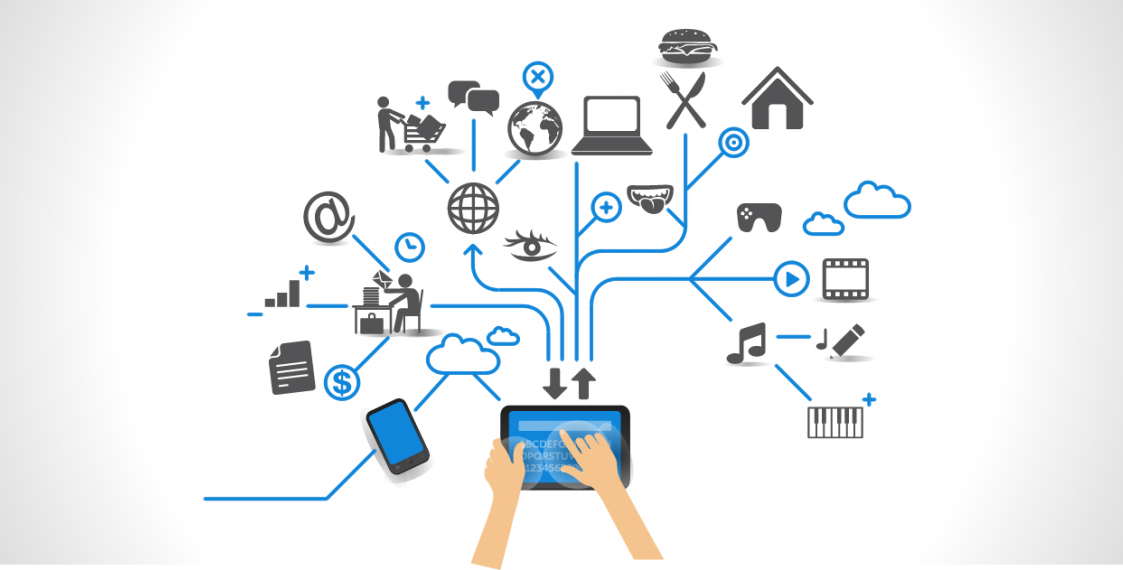
\includegraphics[scale=0.4]{figures/iot_scheme.png}
	\caption{Схематичное представление IoT}
	\label{fig:subject:iot:scheme}
\end{figure}

4 примера умных интернет вещей:
\begin{itemize}
	\item если вы уйдете из дома без кошелька, он сообщит вам об этом по телефону, а сенсор на ошейнике кота сообщит координаты,если кот сбежал далеко от дома;
	\item если вы забыли выключить утюг или телевизор, не нужно идти домой проверять: они сами доложат свой статус;
	\item когда закончился кофе или стиральный порошок, заказать его можно одним нажатием на кнопку;
	\item интернет-вещи напомнят, когда нужно поливать цветы, а целая система, подключенная к вашему огороду, подскажет, когда нужно полить грядки и включить поливающее оборудование;
\end{itemize}

Наше световое оборудование, поставляемое вместе с мобильным приложением, как раз подходит под описание интернета вещей. Данные устройства (гирлянды), обладают wi-fi модулями для связи с мобильны приложением и получением команд от него, а также для связи с другими гирляндами. Само приложение обладает возможностью объединения гирлянд в группы, для последующего взаимодействия сразу с несколькими гирляндами (например при внешнем украшении дома). 